\section{Schließende Statistik}

\begin{bonus}{Aufgabe der schließenden Statistik}
    Die \emph{schließende Statistik} befasst sich mit dem Rückschluß von einer Stichprobe auf die Grundgesamtheit.
    Es muss eine repräsentative (d.h. nur zufallsbeeinflusste) Stichprobe aus der Grundgesamtheit gezogen werden.

    Grundlage der schließenden Statistik ist die Wahrscheinlichkeitsrechnung.
\end{bonus}

\subsection{Grundbegriffe}

\begin{defi}{Grundgesamtheit}
    Unter einer Grundgesamtheit verstehen wir die Gesamtheit gleichartiger Objekte oder Elemente, die hinsichtlich eines bestimmten Merkmals untersucht werden sollen.

    Das interessierende Merkmal beschreiben wir dabei durch eine Zufallsvariable $X$.
\end{defi}

\begin{defi}{Stichprobe}
    Eine Stichprobe vom Umfang $n$ der Zufallsvariablen $X$ ist die Beobachtung von $n$ unabhängigen, identisch verteilten Zufallsvariablen $X_1, \ldots, X_n$.

    $X_1, \ldots, X_n$ nennt man \emph{Stichprobenvariablen}, die beobachteten Werte $x_1, \ldots, x_n$ die \emph{Stichprobenwerte}.
\end{defi}

\subsection{Punktschätzungen}

\begin{defi}{Schätzfunktion}
    Eine Funktion $g(X_1, \ldots, X_n)$ der Stichprobenvariablen heißt \emph{Stichprobenfunktion} und ist wieder eine zufällige Variable.

    Wird die Stichprobenfunktion zur Schätzung des Parameters $\theta$ verwendet, so heißt sie \emph{Schätzfunktion} oder kurz \emph{Schätzer} für $\theta$ und wird mit $\hat{\theta}$ bezeichnet.

    Eine Schätzfunktion $\hat{\theta}$ für den Parameter $\theta$ heißt \emph{erwartungstreu}, wenn gilt:
    \[
        \Mean(\hat{\theta}) = \theta
    \]

    Sie heißt \emph{konsistent}, wenn ihre Varianz mit wachsendem Stichprobenumfang $n$ gegen $0$ strebt:
    \[
        \lim_{n \to \infty} \Var(\hat{\theta}) = 0
    \]
\end{defi}

\begin{example}{Schätzung des Erwartungswertes}
    Das arithmetische Mittel ist eine \emph{erwartungstreue} und \emph{konsistente} Schätzfunktion des Erwartungswertes von $X$.

    Es gilt (Erwartungstreue):
    \[
        \Mean(\conj{X}) = \Mean \left(\frac{1}{n} \sum_{i=1}^n X_i \right) = \frac{1}{n} \Mean \left(\sum_{i=1}^n X_i \right) = \frac{1}{n} \sum_{i=1}^n \Mean(X_i) = \frac{1}{n} \cdot n \cdot \mu = \mu
    \]
    und (Konsistenz):\footnote{Hier werden unter anderem der zentrale Grenzwertsatz und das starke Gesetz der großen Zahlen angewendet.}
    \[
        \Var(\conj{X}) = \Var \left(\frac{1}{n} \sum_{i=1}^n X_i \right) = \frac{1}{n^2} \Var \left( \sum_{i=1}^n X_i \right) = \frac{1}{n^2} \sum_{i=1}^{n} \Var(X_i) = \frac{1}{n^2} \cdot n \cdot \sigma^2 = \frac{\sigma^2}{n}
    \]
\end{example}

\begin{example}{Schätzung der Varianz}
    Die Stichprobenvarianz ist eine \emph{erwartungstreue} und \emph{konsistente} Schätzfunktion der Varianz von $X$.

    Es gilt (Erwartungstreue):
    \begin{alignat*}{1}
        \Mean(S^2) & = \Mean \left( \frac{1}{n-1} \sum_{i=1}^{n} (X_i - \conj{X}) \right)^2                                                          \\
                   & = \Mean \left( \frac{1}{n-1} \sum_{i=1}^{n} (X_i - \mu)^2 - \frac{n}{n-1} (\conj{X} - \mu)^2 \right)                            \\
                   & = \ldots                                                                                                                        \\
                   & = \frac{1}{n-1} \cdot \sum_{i=1}^{n} \Mean \left( (X_i - \mu)^2 \right) - \frac{n}{n-1} \Mean \left( (\conj{X} - \mu)^2 \right) \\
                   & = \frac{n}{n-1} \cdot \sigma^2 - \frac{n}{n-1} \cdot \frac{\sigma^2}{n}                                                         \\
                   & = \frac{n-1}{n-1} \cdot \sigma^2                                                                                                \\
                   & = \sigma^2
    \end{alignat*}

    Auf einen Beweis der Konsistenz wird hier verzichtet.
\end{example}

\begin{example}{Schätzfunktion (Erwartungstreue)}
    Die von einer Maschine für einen bestimmten Arbeitsvorgang benötigte Zeit sei eine Zufallsvariable $X$, für deren Dichtefunktion in Abhängigkeit von einem $\theta \in [0, 2]$ die Gestalt
    \[
        f(x;\theta) =
        \begin{cases}
            \theta + 2(1-\theta)\cdot x & \text{für} \ x \in [0,1] \\
            0                           & \text{sonst}
        \end{cases}
    \]
    unterstellt wird.
    Zu $X$ liege eine einfache Stichprobe $X_1, \ldots , X_n$ (die $X_i$ sind unabhängig) vor.\

    \begin{enumerate}[\alph*)]
        \item Zeigen Sie, dass die Schätzfunktionen
              \begin{enumerate}[i)]
                  \item $\hat{\Theta}_1 = 4 - \frac{6}{n} \sum_{i=1}^{n} X_i$
                  \item $\hat{\Theta}_2 = 3 - \frac{6}{n} \sum_{i=1}^{n} X_i^2$
              \end{enumerate}
              erwartungstreu für $\theta$ sind.
        \item Überprüfen Sie zusätzlich, ob $\hat{\Theta}_1$ konsistent für $\theta$ ist.
    \end{enumerate}

    \exampleseparator

    a) i) Wir wissen, dass $\hat{\Theta}_1$ genau dann erwartungstreu ist, wenn $\Mean(\hat{\Theta}_1) = \theta$ gilt.

    Offensichtlich ist:
    \begin{alignat*}{1}
        \Mean\left( \hat{\Theta}_1 \right) & = \Mean\left( 4 - \frac{6}{n} \sum_{i=1}^{n} X_i \right)                                       \\
                                           & = 4 - \frac{6}{n} \cdot \sum_{i=1}^{n}  \Mean (X_i)                                            \\
                                           & = 4 - 6 \Mean\left( X \right)                                                                  \\
                                           & = 4 - 6 \int_{-\infty}^{\infty} xf(x) \diff x                                                  \\
                                           & = 4 - 6 \left(  \int_{0}^{1} x\cdot \left( \theta + 2(1-\theta)\cdot x \right) \diff x \right) \\
                                           & = \theta
    \end{alignat*}
    \qed

    ii) Wir wissen, dass $\hat{\Theta}_2$ genau dann erwartungstreu ist, wenn $\Mean(\hat{\Theta}_2) = \theta$ gilt.

    Offensichtlich ist:
    \begin{alignat*}{1}
        \Mean\left( \hat{\Theta}_2 \right) & = \Mean\left( 3 - \frac{6}{n} \sum_{i=1}^{n} X_i^2   \right)                \\
                                           & = 3 - \frac{6}{n} \Mean\left( \sum_{i=1}^{n} X_i^2   \right)                \\
                                           & = 3 - 6 \Mean ( X^2 )                                                       \\
                                           & = 3 - 6 \int_{-\infty}^{\infty} x^2f(x) \diff x                             \\
                                           & = 3 - 6 \int_{0}^{1} x^2 \left( \theta + 2(1-\theta)\cdot x \right) \diff x \\
                                           & = \theta
    \end{alignat*}
    \qed
\end{example}

\begin{example}{Schätzfunktion (Konsistenz)}
    b) Wir wissen, dass $\hat{\Theta}_1$ genau dann konsistent ist, wenn $\lim_{n\to\infty}\Var(\hat{\Theta}_1) = 0$ gilt.

    Offensichtlich gilt:
    \begin{alignat*}{1}
        \lim_{n\to\infty}\Var(\hat{\Theta}_1) & = \lim_{n\to\infty}\Var(\hat{\Theta}_1)                                                    \\
                                              & = \lim_{n\to\infty}\Var\left(4 - \frac{6}{n} \sum_{i=1}^{n} X_i\right)                     \\
                                              & = \lim_{n\to\infty}\left( \frac{6}{n} \right)^2 \cdot \Var\left( \sum_{i=1}^{n} X_i\right) \\
                                              & = 36 \cdot \lim_{n\to\infty}\frac{1}{n^2} \cdot \sum_{i=1}^{n} \Var (X_i)                  \\
                                              & = 36 \cdot \lim_{n\to\infty}\frac{1}{n^2} \cdot  n \cdot  \Var (X)                         \\
                                              & = 36 \cdot \lim_{n\to\infty}\frac{1}{n} \cdot  \Var (X)                                    \\
                                              & = 36 \cdot 0                                                                               \\
                                              & = 0
    \end{alignat*}
    \qed
\end{example}

\begin{algo}{Maximum-Likelihood-Methode}
    Bei der \emph{Maximum-Likelihood-Methode} wird von einer Zufallsvariablen $X$ ausgegangen, deren Dichte- bzw. Wahrscheinlichkeitsfunktion $f$ von einem unbekannten Parameter $\theta$ abhängig ist.

    Liegt eine einfache Zufallsstichprobe mit $n$ Realisierungen $x_1, \ldots, x_n$ von $n$ unabhängig und identisch verteilten Zufallsvariablen $X_1, \ldots, X_n$ vor, so lässt sich die gemeinsame Dichtefunktion bzw. Wahrscheinlichkeitsfunktion wie folgt faktorisieren:
    \[
        f(x_1, x_2, \ldots, x_n ; \theta) = \prod_{i=1}^n f(x_i ; \theta)
    \]

    Statt nun für einen festen Parameter $\theta$ die Dichte für beliebige Werte $x_1, \ldots, x_n$ auszuwerten,  kann umgekehrt für beobachtete und somit feste Realisierungen $x_1, \ldots, x_n$ die gemeinsame Dichte als Funktion von $\theta$ interpretiert werden.
    Dies führt zur Likelihood-Funktion:
    \[
        L(\theta) = \prod_{i=1}^n f(x_i ; \theta)
    \]
    Wird diese Funktion in Abhängigkeit von $\theta$ maximiert, also:\footnote{Dies gilt meist. Manchmal ist $L$ aber nicht differenzierbar.}
    \[
        \frac{\partial L}{\partial \theta} = 0\footnote{Beachte, dass auch $\frac{\partial^2 L}{\partial \theta^2} < 0$ gelten muss!}
    \]
    so erhält man die Maximum-Likelihood-Schätzung für den unbekannten Parameter $\theta$.

    Es wird also der Wert von $\theta$ gesucht, bei dem die Stichprobenwerte die größte Dichte- bzw. Wahrscheinlichkeitsfunktion haben.
    Es ist naheliegend, einen Parameterwert $\theta$ als umso plausibler anzusehen, je höher die Likelihood.

    Da das Ableiten bei Dichtefunktionen mit komplizierten Exponentenausdrücken sehr aufwändig werden kann, wird häufig die logarithmierte Likelihood-Funktion  verwendet, da sie auf Grund der Monotonie des Logarithmus ihr Maximum an derselben Stelle wie die nichtlogarithmierte Dichtefunktion besitzt, jedoch einfacher zu berechnen ist:
    \[
        L^*(\theta) = \log \prod_{i=1}^n f(x_i ; \theta) = \sum_{i=1}^n \log f(x_i ; \theta)
    \]

    Die Maximum-Likelihood-Methode liefert nicht immer erwartungstreue Schätzer.
\end{algo}

\begin{example}{Maximum-Likelihood-Methode}
    Aus Erfahrung sei bekannt, dass die Brenndauer einer Glühbirne einer bestimmten Sorte durch eine stetig verteilte Zufallsvariable $X$ mit der Dichte
    \[
        f(x) =
        \begin{cases}
            2\theta \cdot x \cdot e^{-\theta x^2} & \text{für} \ x > 0 \\
            0                                     & \text{sonst}
        \end{cases}
    \]
    beschrieben werden kann.
    Schätzen Sie das für diese Sorte passende $\theta$ aufgrund der folgenden 15 Brenndauern (in 1000 Stunden) mittels der Maximum-Likelihood-Methode:

    \begin{center}
        \begin{tabular}{CCCCC}
            1.5 & 1   & 2   & 1   & 1.5 \\
            1   & 2   & 0.5 & 2.5 & 1.5 \\
            1.5 & 1.5 & 1.5 & 2   & 1.5
        \end{tabular}
    \end{center}

    \exampleseparator

    Es gilt:
    \[
        L(\theta) = \prod_{i=1}^{n} f(x_i) = \prod_{i=1}^{n} 2\theta \cdot x_i \cdot e^{-\theta x_i^2} = (2 \theta)^n \cdot e^{-\theta \cdot \sum_{i=1}^{n} x_i^2}  \cdot \prod_{i=1}^{n} x_i
    \]

    Damit erhalten wir $L^*(\theta)$ mit:
    \[
        L^*(\theta) = \ln L(\theta) = n \cdot \ln 2\theta + \left( -\theta \cdot \sum_{i=1}^{n} x_i^2 \right) \cdot \cancel{\ln e} + \ln \prod_{i=1}^{n} x_i = n (\ln 2 + \ln \theta) - \theta \cdot \sum_{i=1}^{n} x_i^2 + \ln \prod_{i=1}^{n} x_i
    \]

    \[
        \implies \quad \frac{\partial L^*}{\partial \theta} = \frac{n}{\theta} - \sum_{i=1}^{n} x_i^2 \quad \implies \quad \frac{\partial L^*}{\partial \theta} = 0 \quad \iff \quad \theta = \frac{n}{\sum_{i=1}^{n} x_i^2}
    \]

    Damit ist $\theta = \frac{n}{\sum_{i=1}^{n} x_i^2}$ ein potentieller Schätzer für $\theta$.

    Natürlich müssen wir überprüfen, ob es sich um ein Maximum handelt.
    Es gilt offensichtlich:
    \[
        \frac{\partial^2 L^*(\theta)}{\partial \theta^2} = \frac{-n}{\theta^2} < 0 \quad \checkmark
    \]

    Damit haben wir einen Schätzer und es gilt:
    \[
        \theta = \frac{n}{\sum_{i=1}^{n} x_i^2} = \frac{15 \cdot 4}{149} = \frac{60}{149} \approx 0.403
    \]
    \qed
\end{example}

\subsection{Intervallschätzungen}

\begin{defi}{Konfidenzintervall und Konfidenzniveau}
    Sei $X_1, \ldots, X_n$ eine Stichprobe zu einer Verteilung mit Parameter $\theta$ und $0 < \alpha < 1$.

    Ist dann
    \[
        I_n := [ c_u, c_o ]
    \]
    ein Intervall, das von der Stichprobe abhängt und gilt
    \[
        P( \theta \in I_n ) \geq 1 - \alpha
    \]
    dann nennt man $I_n$ \emph{Konfidenzintervall} für $\theta$ mit dem \emph{Konfidenzniveau} $1 - \alpha$.\footnote{Wenn ihr über Konfidenzintervalle und deren beschriebene Parameter redet, formuliert nicht den Satz: \enquote{Der Parameter liegt zu $n\%$ im Konfidenzintervall.} Entweder liegt der Parameter im Intervall, oder nicht.}

    Typische Werte für $\alpha$ sind $\alpha = 0.05$, $\alpha = 0.01$ oder $\alpha = 0.001$.

    Kann man ein Konfidenzintervall von oben und unten begrenzen, spricht man von einem \emph{zweiseitigen Konfidenzintervall} mit
    \[
        I_n = [ c_u, c_o ]
    \]

    Kann man ein Konfidenzintervall nur von einer Seite begrenzen, spricht man von einem \emph{einseitigen Konfidenzintervall} mit entweder
    \[
        I_n = \left[ c_u, \infty \right) \quad \text{(nach unten beschränkt)}
            \]
            oder
            \[
            I_n = \left( -\infty, c_o \right] \quad \text{(nach oben beschränkt)}
    \]
\end{defi}

\begin{bonus}{Berechnung von Intervallen einer Standardnormalverteilung}
    Sei $0 < p < 1$ eine vorgegebene Wahrscheinlichkeit.

    Dann sei $u_p$ das zur Wahrscheinlichkeit $p$ gehörige Quantil (obere Schranke) mit
    \[
        \Phi(u_p) = p
    \]

    Es gilt:
    \[
        u_{1-p} = -u_p \quad \iff \quad u_p = - u_{1-p}
    \]

    Der Wert von $u_p$ kann dann aus folgender Tabelle abgelesen werden:
    \begin{center}
        \begin{tabular}{|C|C||C|C|}
            \hline
            p     & u_p   & p     & u_p    \\
            \hline
            0.90  & 1.282 & 0.1   & -1.282 \\
            0.95  & 1.645 & 0.05  & -1.645 \\
            0.975 & 1.960 & 0.025 & -1.960 \\
            0.99  & 2.326 & 0.01  & -2.326 \\
            0.995 & 2.576 & 0.005 & -2.576 \\
            0.999 & 3.090 & 0.001 & -3.090 \\
            \hline
        \end{tabular}
    \end{center}

    Für zu berechnende Intervalle gilt dann:
    \begin{enumerate}
        \item Einseitige Abgrenzung nach oben:
              \[
                  P( U \leq c) = \Phi(c) = p
              \]
              \[
                  \Phi(c) = p \implies c = u_p
              \]
        \item Einseitige Abgrenzung nach unten:
              \[
                  P( U \geq c) = 1 -  P( U \leq c) = 1 - \Phi(c) = 1 - p
              \]
              \[
                  \Phi(c) = 1 - p \implies c = u_{1-p}
              \]
        \item \hl{Zweiseitige (symmetrische) Abgrenzung}:
              \[
                  \mhl{P( -c \leq U \leq c) = 2 \cdot \Phi(c) - 1 = p}
              \]
              \[
                  \mhl{\Phi(c) = \frac{1}{2} (1+p) = u_{\nicefrac{(1+p)}{2}}}
              \]
    \end{enumerate}
\end{bonus}

\begin{algo}{Konfidenzintervalle für den unbekannten Erwartungswert einer Normalverteilung bei bekannter Varianz}
    $X$ sei eine normalverteilte Zufallsvariable mit \emph{unbekanntem} Erwartungswert $\mu$ und \emph{bekannter} Varianz $\sigma^2$.

    Wir wissen, dass das arithmetische Mittel ein Schätzer für den Erwartungswert $\mu$ ist:
    \[
        \conj{X} = \frac{1}{n} \sum_{i=1}^{n} X_i
    \]

    Die normierte Zufallsvariable
    \[
        \mhl{U = \sqrt{n} \cdot \frac{\conj{X} - \mu}{\sigma}}
    \]
    ist dann standardnormalverteilt.


    Für $U$ lässt sich dann schrittweise ein Konfidenzintervall konstruieren:
    \begin{enumerate}
        \item Wähle ein bestimmtes Konfidenzniveau $\gamma = 1 - \alpha$
        \item Die Zufallsvariable $U$ soll dann mit der gewählten Wahrscheinlichkeit $\gamma$ einen Wert in dem \emph{symmetrischen} Intervall $-c \leq U \leq c$ annehmen, also:
              \[
                  \mhl{P(-c \leq U \leq c) = \gamma = 1 - \alpha}
              \]
        \item Mit dem vorgegebenen Konfidenzniveau $\gamma$ können wir dann das Intervall wie folgt berechnen:
              \begin{alignat*}{3}
                               & -c                                                                    &  & \leq U                                            &  & \leq c                                                                     \\
                  \equiv \quad & -u_{\gamma}                                                           &  & \leq U                                            &  & \leq u_{\gamma}                                                            \\
                  \equiv \quad & -u_{\nicefrac{(1+\gamma)}{2}}                                         &  & \leq U                                            &  & \leq u_{\nicefrac{(1+\gamma)}{2}}                                          \\
                  \equiv \quad & -u_{\nicefrac{(1+1 - \alpha)}{2}}                                     &  & \leq U                                            &  & \leq u_{\nicefrac{(1+1 - \alpha)}{2}}                                      \\
                  \equiv \quad & -u_{1 - \nicefrac{\alpha}{2}}                                         &  & \leq U                                            &  & \leq u_{1 - \nicefrac{\alpha}{2}}                                          \\
                  \equiv \quad & -u_{1 - \nicefrac{\alpha}{2}}                                         &  & \leq \sqrt{n} \cdot \frac{\conj{X} - \mu}{\sigma} &  & \leq u_{1 - \nicefrac{\alpha}{2}}                                          \\
                  \equiv \quad & \conj{X} - u_{1 - \nicefrac{\alpha}{2}} \cdot \frac{\sigma}{\sqrt{n}} &  & \leq \mu                                          &  & \leq \conj{X} + u_{1 - \nicefrac{\alpha}{2}} \cdot \frac{\sigma}{\sqrt{n}}
              \end{alignat*}
              \[
                  \implies P \left( \conj{X} - u_{1 - \nicefrac{\alpha}{2}} \cdot \frac{\sigma}{\sqrt{n}} \leq \mu \leq \conj{X} + u_{1 - \nicefrac{\alpha}{2}} \cdot \frac{\sigma}{\sqrt{n}} \right) = \gamma = 1 - \alpha
              \]
        \item Die Berechnung der Intervallgrenzen erfolgt dann anhand einer konkreten Stichprobe.

              Das Konfidenzintervall
              \[
                  \mhl{\conj{X} - u_{1 - \nicefrac{\alpha}{2}} \cdot \frac{\sigma}{\sqrt{n}} \leq \mu \leq \conj{X} + u_{1 - \nicefrac{\alpha}{2}} \cdot \frac{\sigma}{\sqrt{n}}}
              \]
              enthält den unbekannten Erwartungswert $\mu$ der normalverteilten Grundgesamtheit mit einem Konfidenzniveau von $\gamma$.
    \end{enumerate}
\end{algo}

\begin{example}{Konfidenzintervalle für den unbekannten Erwartungswert einer Normalverteilung bei bekannter Varianz}
    12 Versuchsflächen wurden mit einer neuen Weizensorte bestellt.
    Diese Flächen erbrachten folgende Hektarerträge (in Doppelzentner):

    \begin{center}
        \begin{tabular}{cccccccccccc}
            35.6 & 33.7 & 37.8 & 31.2 & 37.2 & 43.1 & 35.8 & 36.6 & 37.1 & 34.9 & 35.6 & 34.0
        \end{tabular}
    \end{center}

    Aus Erfahrung weiß man, dass die Hektarerträge als eine Realisierung unabhängiger $\mathcal{N}(\mu, (\sqrt{3})^2)$ - verteilter Zufallsvariablen angesehen werden können.

    Geben Sie für den Erwartungswert $\mu$ ein konkretes Konfidenzintervall zum Niveau $0.95$ an.

    \exampleseparator

    Wir wissen, dass gilt:
    \[
        X := \text{Hektarerträge (in Doppelzentner)} \sim \mathcal{N}(\mu, (\sqrt{3})^2)
    \]

    Ein geeigneter Schätzer für $\mu$ ist bekanntermaßen
    \[
        \conj{X} = \frac{1}{n} \cdot \sum_{i=1}^{n} x_i
    \]

    Für unsere Verteilung sind die relevanten Kennzahlen übrigens:
    \[
        \conj{X} = \frac{1}{12} \cdot 432.6 = 36.05 \quad \land \quad \sigma^2 = 3 \implies \sigma = \sqrt{3}
    \]

    Die normierte Zufallsvariable $U$ mit
    \[
        U = \sqrt{n} \cdot \frac{\conj{X} - \mu}{\sigma}
    \]
    ist dann standarnormalverteilt mit $\mathcal{N}(0, 1)$.

    Es muss gelten:
    \[
        P(-c \leq U \leq c) = \gamma = 1 - \alpha
    \]

    Damit gilt:
    \begin{alignat*}{2}
                     & P(\conj{X} - u_{1 - \nicefrac{\alpha}{2}} \cdot \frac{\sigma}{\sqrt{n}} \leq \mu \leq \conj{x} + u_{1 - \nicefrac{\alpha}{2}} \cdot \frac{\sigma}{\sqrt{n}}) &  & = \gamma \\
        \equiv \quad & P(36.05 - 1.960 \cdot \frac{1}{2} \leq \mu \leq 36.05 + 1.960 \cdot \frac{1}{2})                                                                             &  & = 0.95   \\
        \equiv \quad & P(35.07 \leq \mu \leq 37.03)                                                                                                                                 &  & = 0.95
    \end{alignat*}

    Damit erhalten wir unser Konfidenzintervall $I_{12}$ mit
    \[
        I_{12} = [35.07, 37.03]
    \]
    \qed
\end{example}

\begin{defi}{Chi-Quadrat-Verteilung}
    $X_1, \ldots, X_n$ seien mit $n$ mit $\mathcal{N}(0, 1)$ verteilte, stochastisch unabhängige Zufallsvariablen.

    Betrachte die stetige Zufallsvariable $Z$ mit Wertebereich $z \geq 0$:
    \[
        Z = X_1^2 + \ldots + X_n^2
    \]
    $Z$ ist dann \emph{Chi-Quadrat-verteilt} mit der Anzahl der Freiheitsgraden $n$, man schreibt $Z \sim \chi^2_n$.

    Die Dichte- und Verteilungsfunktion der Chi-Quadrat-Verteilung sind an dieser Stelle nicht wirklich relevant.
    In den Teilen, in denen sie genutzt wird, muss lediglich der jeweilige Wert eines oder mehrerer $\chi^2_n (z)$ aus einer Tabelle abgelesen werden.

    Eigenschaften der Chi-Quadrat-Verteilung:
    \begin{itemize}
        \item Die Dichtefunktion ist asymmetrisch.
        \item Die Dichtefunktion ist für $n \in \{ 1, 2 \}$ streng monoton fallend.
        \item Die Dichtefunktion besitzt für $n > 2$ ein absolutes Maximum bei $z_{\max} = n-2$.
        \item Für große Freiheitsgrade ($n > 1000$) lässt sich die Chi-Quadrat-Verteilung durch eine Normalverteilung $\mathcal{N} (n, 2n)$ annähern.
    \end{itemize}
\end{defi}

\begin{example}{Chi-Quadrat-Verteilung}
    \begin{center}
        \begin{tikzpicture}
            \begin{axis}[%
                    width=\linewidth,
                    height=0.45\linewidth,
                    xlabel = $z$,
                    ylabel = $f(z)$,
                    samples = 200,
                    restrict y to domain = 0:0.5,
                    domain = 0.01:15]
                \foreach \n in {1,...,8} {%
                        \addplot+[mark={}] gnuplot[raw gnuplot] {%
                                isint(x) = (int(x)==x);
                                log2 = 0.693147180559945;
                                chisq(x,n)=n<=0||!isint(n)?1/0:x<=0?0.0:exp((0.5*n-1.0)*log(x)-0.5*x-lgamma(0.5*n)-n*0.5*log2);
                                set xrange [1.00000e-5:15.0000];
                                set yrange [0.00000:0.500000];
                                samples=200;
                                plot chisq(x,\n)};
                        \addlegendentryexpanded{$n = \n$}}
            \end{axis}
        \end{tikzpicture}
    \end{center}
\end{example}

\begin{bonus}{Anzahl der Freiheitsgrade}
    Schätzungen statistischer Parameter können auf unterschiedlichen Mengen an Informationen oder Daten basieren.
    Die Anzahl unabhängiger Information, die in die Schätzung eines Parameters einfließen, wird als \emph{Anzahl der Freiheitsgrade} bezeichnet.

    Im Allgemeinen sind die Freiheitsgrade einer Schätzung eines Parameters gleich der Anzahl unabhängiger Einzelinformationen, die in die Schätzung einfließen, abzüglich der Anzahl der zu schätzenden Parameter, die als Zwischenschritte bei der Schätzung des Parameters selbst verwendet werden.

    Beispielsweise fließen in die Berechnung der Stichprobenvarianz $n$ Werte mit ein.
    Dennoch lautet die Anzahl der Freiheitsgrade $n-1$, da als Zwischenschritt der Mittelwert geschätzt wird und somit ein Freiheitsgrad verloren geht.
\end{bonus}

\begin{algo}{Konfidenzintervalle für die unbekannte Varianz einer Normalverteilung}
    $X$ sei eine normalverteilte Zufallsvariable mit \emph{unbekanntem} Erwartungswert $\mu$ und \emph{unbekannter} Varianz $\sigma^2$.

    Wir wissen, dass das Stichprobenmittel ein Schätzer für die Varianz $\sigma^2$ ist:
    \[
        S^2 = \frac{1}{n-1} \sum_{i=1}^n (X_i - \conj{X})^2
    \]

    Die Variable
    \[
        \mhl{Z = (n-1) \cdot \frac{S^2}{\sigma^2} = \frac{1}{\sigma^2} \sum_{i=1}^n (X_i - \conj{X})^2 = \sum_{i=1}^n (\frac{X_i - \conj{X}}{\sigma})^2}
    \]
    ist dann Chi-Quadrat-verteilt mit $f = n-1$ Freiheitsgraden.\footnote{$n-1$ Freiheitsgrade statt $n$, da hier $\mu$ über $\conj{X}$ der Stichprobe geschätzt werden muss.}

    Für $Z$ lässt sich dann schrittweise ein Konfidenzintervall konstruieren:
    \begin{enumerate}
        \item Wähle ein bestimmtes Konfidenzniveau $\gamma = 1 - \alpha$
        \item Die Zufallsvariable $Z$ soll dann mit der gewählten Wahrscheinlichkeit $\gamma$ einen Wert in dem Intervall $c_1 \leq Z \leq c_2$ annehmen, also:
              \[
                  \mhl{P(c_1 \leq Z \leq c_2) = \gamma = 1 - \alpha}
              \]
        \item Mit dem vorgegebenen Konfidenzniveau $\gamma$ können wir dann das Intervall wie folgt berechnen:
              \begin{alignat*}{3}
                               & c_1                                                            &  & \leq Z                                &  & \leq c_2                                                         \\
                  \equiv \quad & \chi^2_{n-1} (\nicefrac{\alpha}{2})                            &  & \leq Z                                &  & \leq \chi^2_{n-1} (1 - \nicefrac{\alpha}{2})                     \\
                  \equiv \quad & \chi^2_{n-1} (\nicefrac{\alpha}{2})                            &  & \leq (n-1) \cdot \frac{S^2}{\sigma^2} &  & \leq \chi^2_{n-1} (1 - \nicefrac{\alpha}{2})                     \\
                  \equiv \quad & (n-1) \cdot \frac{S^2}{\chi^2_{n-1}(1 - \nicefrac{\alpha}{2})} &  & \leq \sigma^2                         &  & \leq (n-1) \cdot \frac{S^2}{\chi^2_{n-1} (\nicefrac{\alpha}{2})}
              \end{alignat*}
              \[
                  \implies P \left( (n-1) \cdot \frac{S^2}{\chi^2_{n-1}(1 - \nicefrac{\alpha}{2})} \leq \sigma^2 \leq (n-1) \cdot \frac{S^2}{\chi^2_{n-1} (\nicefrac{\alpha}{2})} \right) = \gamma = 1 - \alpha
              \]
        \item Die Berechnung der Intervallgrenzen erfolgt dann anhand einer konkreten Stichprobe.

              Das Konfidenzintervall
              \[
                  \mhl{(n-1) \cdot \frac{S^2}{\chi^2_{n-1}(1 - \nicefrac{\alpha}{2})} \leq \sigma^2 \leq (n-1) \cdot \frac{S^2}{\chi^2_{n-1} (\nicefrac{\alpha}{2})}}
              \]
              enthält die unbekannte Varianz $\sigma^2$ der normalverteilten Grundgesamtheit mit einem Konfidenzniveau $\gamma$.

              Durch Radizieren erhält man ein entsprechendes Konfidenzintervall für $\sigma$.
    \end{enumerate}
\end{algo}

\begin{example}{Konfidenzintervalle für die unbekannte Varianz einer Normalverteilung}
    Das Gewicht $X$, das ein Apfel einer bestimmten Sorte hat, sei normalverteilt.
    Die Untersuchung einer Stichprobe vom Umfang $n = 10$ ergab einen Mittelwert $\conj{x} = 98 \si{g}$ und eine empirische Standardabweichung $s = 0.75 \si{g}$.
    Geben Sie den Bereich an, in dem die Varianz mit 95\%-iger Sicherheit liegt.

    \exampleseparator

    Wir wissen, dass gilt:
    \[
        X \sim \mathcal{N}(\mu, \sigma^2)
    \]

    Ein geeigneter Schätzer für $\Var(X) = \sigma^2$ ist bekanntermaßen
    \[
        s^2 = \frac{1}{n-1} \cdot \sum_{i=1}^{n} (x_i - \conj{x})^2
    \]

    Für unsere Verteilung gilt dann:
    \[
        s^2 = 0.75^2 = 0.5625
    \]

    Die Zufallsvariable $Z$ mit
    \[
        Z = (n-1) \cdot \frac{s^2}{\sigma^2} = \frac{1}{\sigma^2} \cdot \sum_{i=1}^{n} (x_i - \conj{x})^2 = \sum_{i=1}^{n} \left(\frac{x_i - \conj{x}}{\sigma}\right)^2
    \]
    ist dann $\chi^2$-verteilt mit $n-1$ Freiheitsgraden.

    Es muss gelten:
    \[
        P(c_1 \leq Z \leq c_2) = \gamma = 1 - \alpha
    \]
    Damit gilt:
    \begin{alignat*}{2}
                     & P((n-1) \cdot \frac{s^2}{\chi^2_{n-1} \left( 1 - \frac{\alpha}{2} \right)} \leq  \sigma^2 \leq (n-1) \cdot \frac{s^2}{\chi^2_{n-1} \left(\frac{\alpha}{2} \right)}) & = \gamma \\
        \equiv \quad & P(9 \cdot \frac{0.5625}{\chi^2_{9} \left( 0.975 \right)}                   \leq \sigma^2  \leq 9 \cdot \frac{0.5625}{\chi^2_9 \left(0.025 \right)})                 & = 0.95   \\
        \equiv \quad & P(9 \cdot \frac{0.5625}{19.02}                                             \leq \sigma^2  \leq 9 \cdot \frac{0.5625}{2.70})                                         & = 0.95   \\
        \equiv \quad & P(0.2662                                                                   \leq \sigma^2  \leq 1.875)                                                               & = 0.95   \\
    \end{alignat*}

    Damit erhalten wir unser Konfidenzintervall $I_{10}$ mit
    \[
        I_{10} = [0.2662, 1.875]
    \]
    \qed
\end{example}

\begin{defi}{t-Verteilung}
    $X$ und $Y$ seien zwei stochastisch unabhängige Zufallsvariablen mit
    \[
        X \sim \mathcal{N}(0, 1) \quad \land \quad Y \sim \chi^2_n
    \]

    Dann ist die stetige Zufallsvariable $T$ mit
    \[
        T = \frac{T}{\sqrt{\frac{Y}{n}}}
    \]
    \emph{t-verteilt} mit $n$ Freiheitsgraden, man schreibt $T \sim t_n$.

    Die Dichte- und Verteilungsfunktion der t-Verteilung sind an dieser Stelle nicht wirklich relevant.
    In den Teilen, in denen sie genutzt wird, muss lediglich der jeweilige Wert eines oder mehrerer $t_n (t)$ aus einer Tabelle abgelesen werden.

    Eigenschaften der t-Verteilung:
    \begin{itemize}
        \item Die Dichtefunktion ist eine gerade Funktion (achsensymmetrisch).
        \item Die Dichtefunktion besitzt an der Stelle $t_{\max} = 0$ ein absolutes Maximum.
        \item Die Dichtefunktion nähert sich für $t \to \pm \infty$ asymptotisch der $t$-Achse.
        \item Für große Freiheitsgrade ($n > 30$) lässt sich die t-Verteilung durch die Standardnormalverteilung $\mathcal{N}(0, 1)$ annähern.
    \end{itemize}
\end{defi}

\begin{example}{t-Verteilung}
    \begin{center}
        \includegraphics[width=.7\linewidth]{includes/figures/example_t_verteilung}
    \end{center}
\end{example}

\begin{algo}{Konfidenzintervalle für den unbekannten Erwartungswert einer Normalverteilung bei unbekannter Varianz}
    $X$ sei eine normalverteilte Zufallsvariable mit \emph{unbekanntem} Erwartungswert $\mu$ und \emph{unbekannter} Varianz $\sigma^2$.

    Wir wissen, dass das arithmetische Mittel ein Schätzer für den Erwartungswert $\mu$ ist:
    \[
        \conj{X} = \frac{1}{n} \sum_{i=1}^{n} X_i
    \]

    Wir wissen auch, dass die Wurzel des Stichprobenmittels ein Schätzer für die Standardabweichung $\sigma$ ist:
    \[
        S = \sqrt{ \frac{1}{n-1} \sum_{i=1}^n (X_i - \conj{X})^2 }
    \]

    Die normierte Variable
    \[
        \mhl{ T = \sqrt{n} \cdot \frac{\conj{X} - \mu}{S} }
    \]
    ist dann t-verteilt mit $f = n-1$ Freiheitsgraden.

    Für $T$ lässt sich dann schrittweise ein Konfidenzintervall konstruieren:
    \begin{enumerate}
        \item Wähle ein bestimmtes Konfidenzniveau $\gamma = 1 - \alpha$
        \item Die Zufallsvariable $T$ soll dann mit der gewählten Wahrscheinlichkeit $\gamma$ einen Wert in dem \emph{symmetrischen} $-c \leq U \leq c$ annehmen, also:
              \[
                  \mhl{P(-c \leq T \leq c) = \gamma = 1 - \alpha}
              \]
        \item Mit dem vorgegebenen Konfidenzniveau $\gamma$ können wir dann das Intervall wie folgt berechnen:
              \begin{alignat*}{3}
                               & -c                                                                     &  & \leq T                                       &  & \leq c                                                                      \\
                  \equiv \quad & -t_{n-1} (1 - \nicefrac{\alpha}{2})                                    &  & \leq T                                       &  & \leq t_{n-1} (1 - \nicefrac{\alpha}{2})                                     \\
                  \equiv \quad & -t_{n-1} (1 - \nicefrac{\alpha}{2})                                    &  & \leq \sqrt{n} \cdot \frac{\conj{X} - \mu}{S} &  & \leq t_{n-1} (1 - \nicefrac{\alpha}{2})                                     \\
                  \equiv \quad & \conj{X} - t_{n-1} (1 - \nicefrac{\alpha}{2}) \cdot \frac{S}{\sqrt{n}} &  & \leq \mu                                     &  & \leq \conj{X} + t_{n-1} (1 - \nicefrac{\alpha}{2}) \cdot \frac{S}{\sqrt{n}}
              \end{alignat*}
              \[
                  \implies P \left( \conj{X} - t_{n-1} (1 - \nicefrac{\alpha}{2}) \cdot \frac{S}{\sqrt{n}} \leq \mu \leq \conj{X} + t_{n-1} (1 - \nicefrac{\alpha}{2}) \cdot \frac{S}{\sqrt{n}} \right) = \gamma = 1 - \alpha
              \]
        \item Die Berechnung der Intervallgrenzen erfolgt dann anhand einer konkreten Stichprobe.

              Das Konfidenzintervall
              \[
                  \mhl{ \conj{X} - t_{n-1} (1 - \nicefrac{\alpha}{2}) \cdot \frac{S}{\sqrt{n}} \leq \mu \leq \conj{X} + t_{n-1} (1 - \nicefrac{\alpha}{2}) \cdot \frac{S}{\sqrt{n}} }
              \]
              enthält den unbekannten Erwartungswert $\gamma$ der normalverteilten Grundgesamtheit mit einem Konfidenzniveau von $\gamma$.
    \end{enumerate}
\end{algo}

\begin{example}{Konfidenzintervalle für den unbekannten Erwartungswert einer Normalverteilung bei unbekannter Varianz}
    Das Umweltreferat einer Großstadt will Aufschluss darüber gewinnen, wie viele Asbestfasern pro Kubikmeter Luft im Freien in ca. einem Meter Abstand von asbestzementhaltigen Gebäudeteilen zu erwarten sind.
    Bei $n = 14$ diesbezüglichen Messungen traten die Werte
    \begin{center}
        \begin{tabular}{ccccccc}
            980  & 1340 & 610  & 750 & 880  & 1250 & 2410 \\
            1100 & 470  & 1040 & 910 & 1860 & 730  & 820
        \end{tabular}
    \end{center}
    auf, die als Ergebnisse unabhängiger normalverteilter Stichprobenvariablen angesehen werden.

    Führen Sie für den Erwartungswert $\mu$ der Anzahl $X$ der unter den obigen Bedingungen vorhandenen Asbestfasern eine Intervallschätzung zum Konfidenzniveau $0.95$ durch.

    \exampleseparator

    Wir wissen, dass gilt:
    \[
        X \sim \mathcal{N}(\mu, \sigma^2)
    \]

    Geeignete Schätzer für $\mu$ bzw. $\sigma$ sind bekanntermaßen
    \[
        \conj{X} = \frac{1}{n} \cdot \sum_{i=1}^{n} x_i \quad \text{bzw.} \quad S = \sqrt{\frac{1}{n-1} \cdot \sum_{i=1}^{n} (x_i - \conj{x})^2}
    \]

    Für unsere Verteilung gilt dann:
    \[
        \conj{X} = \frac{1}{14} \cdot 15150 = \frac{7575}{7} \quad \text{bzw.} \quad S = \sqrt{\frac{1}{13} \cdot \frac{24126450}{7}} = \frac{5\sqrt{87820278}}{91} \approx 514.9
    \]

    Die Zufallsvariable $T$ mit
    \[
        T = \sqrt{n} \cdot \frac{\conj{X} - \mu}{S}
    \]
    ist dann $t$-verteilt mit $n-1$ Freiheitsgraden.

    Es muss gelten:
    \[
        P(-c \leq T \leq c) = \gamma = 1 - \alpha
    \]

    Damit gilt:
    \begin{alignat*}{2}
                     & P(\conj{X} - t_{n-1} \left( 1-\frac{\alpha}{2} \right) \cdot \frac{S}{\sqrt{n}} \leq  \mu \leq \conj{X} + t_{n-1} \left( -\frac{\alpha}{2} \right) \cdot \frac{s}{\sqrt{n}}) & = \gamma \\
        \equiv \quad & P(\frac{7575}{7} - t_{13} \left( 0.975 \right) \cdot \frac{514.9}{\sqrt{14}} \leq  \mu \leq \frac{7575}{7} + t_{13} \left( 0.975 \right) \cdot \frac{514.9}{\sqrt{14}})      & = 0.95   \\
        \equiv \quad & P(\frac{7575}{7} - 2.160 \cdot \frac{514.9}{\sqrt{14}} \leq  \mu \leq \frac{7575}{7} + 2.160 \cdot \frac{514.9}{\sqrt{14}})                                                  & = 0.95   \\
        \equiv \quad & P(784.897 \leq  \mu \leq 1379.389)                                                                                                                                           & = 0.95   \\
    \end{alignat*}

    Damit erhalten wir unser Konfidenzintervall $I_{14}$ mit
    \[
        I_{14} = [784.897, 1379.389]
    \]
    \qed
\end{example}

\begin{algo}{Konfidenzintervalle für den unbekannten Anteilswert $p$ (Parameter $p$ einer Binomialverteilung)}
    Sei $p = P(A)$ die Wahrscheinlichkeit für ein Ereignis $A$ in einem Bernoulli-Experiment.

    Dann ist
    \[
        X := \text{Anzahl des Eintretens von $A$}
    \]
    bei einer $n$-fachen Ausführung des Bernoulli-Experiments eine \emph{binomialverteilte Zufallsvariable}, die bei umfangreichen Stichproben näherungsweise normalverteilt ist\footnote{Siehe Grenzwertsatz von Moivre und Laplace} mit
    \[
        \Mean(X) = \mu = np \quad \land \quad \Var(X) = \sigma^2 = np(1-p)
    \]

    Eine erwartungstreue Schätzfunktion für $p$ ist:
    \[
        \hat{p} = \frac{X}{n} \quad \implies \quad X = n \cdot \hat{p}
    \]

    Die Zufallsvariable
    \[
        \mhl{ U = \frac{X-\mu}{\sqrt{\Var(\hat{p})}} = \frac{X - np}{\sqrt{n\hat{p}(1-\hat{p})}} = \frac{n\hat{p} - np}{\sqrt{n\hat{p}(1-\hat{p})}}}
    \]
    ist dann näherungsweise standardnormalverteilt.

    Für $p$ lässt sich dann schrittweise ein Konfidenzintervall konstruieren:
    \begin{enumerate}
        \item Wähle ein bestimmtes Konfidenzniveau $\gamma = 1 - \alpha$
        \item Die Zufallsvariable $U$ soll dann mit der gewählten Wahrscheinlichkeit $\gamma$ einen Wert in dem \emph{symmetrischen} $-c \leq U \leq c$ annehmen, also:
              \[
                  \mhl{ P(-c \leq U \leq c) = \gamma = 1 - \alpha }
              \]
        \item Mit dem vorgegebenen Konfidenzniveau $\gamma$ können wir dann das Intervall wie folgt berechnen:
              \begin{alignat*}{3}
                               & -c                                                                          &  & \leq U &  & \leq c                                                                           \\
                  \equiv \quad & \ldots                                                                                                                                                                        \\
                  \equiv \quad & \hat{p} - \frac{u_{1 - \nicefrac{\alpha}{2}}}{n} \sqrt{n\hat{p}(1-\hat{p})} &  & \leq p &  & \leq \hat{p} + \frac{u_{1 - \nicefrac{\alpha}{2}}}{n} \sqrt{n\hat{p}(1-\hat{p})}
              \end{alignat*}
              \[
                  \implies P \left( \hat{p} - \frac{u_{1 - \nicefrac{\alpha}{2}}}{n} \sqrt{n\hat{p}(1-\hat{p})} \leq p \leq \hat{p} + \frac{u_{1 - \nicefrac{\alpha}{2}}}{n} \sqrt{n\hat{p}(1-\hat{p})} \right) = \gamma = 1 - \alpha
              \]
        \item Die Berechnung der Intervallgrenzen erfolgt dann anhand einer konkreten Stichprobe.\footnote{In dieser gilt dann $\hat{p} = \nicefrac{k}{n}$, wobei $k$ die Anzahl der eingetretenen Elemente mit Eigenschaft $A$ darstellt.}

              Das Konfidenzintervall
              \[
                  \mhl{ \hat{p} - \frac{u_{1 - \nicefrac{\alpha}{2}}}{n} \sqrt{n\hat{p}(1-\hat{p})} \leq p \leq \hat{p} + \frac{u_{1 - \nicefrac{\alpha}{2}}}{n} \sqrt{n\hat{p}(1-\hat{p})} }
              \]
              enthält den unbekannten Anteilswert $p$ der binomialverteilten Grundgesamtheit mit einem Konfidenzniveau von $\gamma$.
    \end{enumerate}
\end{algo}

\subsection{Statistische Testverfahren}

\begin{defi}{Hypothesentest}
    Ein \emph{Hypothesentest} dient dazu, anhand vorliegender Beobachtungen eine begründete Entscheidung über die Gültigkeit oder Ungültigkeit einer Hypothese zu treffen.

    Da die vorhandenen Daten Realisierungen von Zufallsvariablen sind, lässt sich meist nicht mit Sicherheit sagen, ob eine Hypothese stimmt oder nicht.
    Man versucht daher, die Wahrscheinlichkeiten für Fehlentscheidungen zu kontrollieren (Signifikanzniveau).
\end{defi}

\begin{algo}{Planung und Durchführung eines Parametertests}
    Die Wahrscheinlichkeitsverteilung einer Zufallsvariablen $X$ sei von der Art her bekannt, enthalte jedoch noch einen oder mehrere unbekannte Parameter.

    \begin{enumerate}
        \item Formulieren der \emph{Nullhypothese} $H_0$ und \emph{Alternativhypothese} $H_1$:
              \begin{itemize}
                  \item Einseitiger Test:
                        \begin{itemize}
                            \item Nullhypothese: $H_0: \theta \leq \theta_0$ bzw. $H_0: \theta \geq \theta_0$
                            \item \emph{einseitige} Alternativhypothese: $H_1: \theta > \theta_0$ bzw. $H_1: \theta < \theta_0$
                        \end{itemize}
                  \item Zweiseitiger Test:
                        \begin{itemize}
                            \item Nullhypothese: $H_0: \theta = \theta_0$
                            \item \emph{zweiseitige} Alternativhypothese: $H_1: \theta \neq \theta_0$
                        \end{itemize}
              \end{itemize}
        \item Festlegung des Signifikantsniveaus $\alpha$.\footnote{$\alpha$ gibt die Wahrscheinlichkeit an, die Nullhypothese abzulehnen, obwohl sie zutrifft. Siehe \emph{Fehler 1. Art}.}
              (typisch: $\alpha = 0.05$, $\alpha = 0.01$, $\alpha = 0.001$)
        \item Bestimmung einer Test- bzw. Prüfvariablen $T = g(X_1, X_2, \ldots, X_n)$\footnote{Stichprobenfunktion, deren Wahrscheinlichkeitsverteilung als bekannt vorausgesetzt werden muss.}
        \item Auf Basis des Signifikantsniveaus $\alpha$ werden kritische Grenzen berechnet, so dass Testvariable $T$ mit Wahrscheinlichkeit $\gamma = 1 - \alpha$ Werte aus jeweiligem Intervall annimmt:
              \begin{itemize}
                  \item Einseitiger Test:
                        \[
                            P(c_u \leq T \leq c_o) = \gamma = 1 - \alpha
                        \]
                  \item Zweiseitiger Test:
                        \[
                            P(T \leq c) = \gamma = 1 - \alpha \quad \text{bzw.} \quad P(T \geq c) = \gamma = 1 - \alpha
                        \]
              \end{itemize}
        \item Berechnung eines Test- bzw. Prüfwertes von $T$ aus einer konkreten Stichprobe:
              \[
                  x_1, \ldots, x_n  \implies \hat{t} = g(x_1, \ldots, x_n)
              \]
        \item Testentscheidung anhand des Wertes von $\hat{t}$:
              \begin{enumerate}
                  \item $\hat{t}$ fällt in den nicht-kritischen Bereich der Testvariablen $T$ (Bereich von $H_0$):
                        \begin{itemize}
                            \item $H_0$ wird nicht verworfen
                            \item Unterschied zwischen Schätzwert $\hat{t}$ und angenommenen Wert $\theta_0$ ist zufallsbedingt.
                        \end{itemize}
                  \item $\hat{t}$ fällt in den kritischen Bereich der Testvariablen $T$ (Bereich von $H_1$):
                        \begin{itemize}
                            \item $H_0$ wird zugunsten der Alternativhypothese $H_1$ verworfen
                            \item Schätzwert $\hat{t}$ weicht \emph{signifikant} von dem angenommenen Wert $\theta_0$ ab.
                        \end{itemize}
              \end{enumerate}
    \end{enumerate}

    \emph{Faustregel:}
    \begin{itemize}
        \item $H_0$ enthält immer das Gleichheitszeichen
        \item $H_0$ nicht verwerfbar, wenn durch Stichprobe gestützt
    \end{itemize}
\end{algo}

\begin{defi}{Fehler 1. Art}
    Eine an sich \emph{richtige Nullhypothese} $H_0$ wird \emph{verworfen}.

    Die Wahrscheinlichkeit für einen Fehler 1. Art wird mit $\alpha$ bezeichnet.

    Über die Entscheidung für ein Signifikanzniveau $\alpha$ wird also auch die Wahrscheinlichkeit für das Auftreten des Fehlers 1. Art festgelegt.
\end{defi}

\begin{defi}{Fehler 2. Art}
    Eine an sich \emph{falsche Nullhypothese} $H_0$ wird \emph{nicht verworfen}.

    Die Wahrscheinlichkeit für einen Fehler 2. Art wird mit $\beta$ bezeichnet.

    Im Gegensatz zum Fehler 1. Art lässt sich die Wahrscheinlichkeit eines Fehler 2. Art meist nicht vorab bestimmen.\footnote{Grund dafür ist, dass die Alternativhypothese im Gegensatz zur Nullhypothese i.d.R. sehr unbestimmter bzw. globaler Natur ist.}

    Zur Berechnung von $\beta$ ist die tatsächliche Verteilung bzw. der tatsächliche Parameter $\theta_1$ nötig.
\end{defi}

\begin{example}{Fehler 1. und 2. Art}
    Es seien zwei Hypothesentests gegeben:
    \begin{itemize}
        \item $\mu_0$ sei zu bestimmen
        \item $H_0$ behaupte in beiden Fällen, dass $\mu_0$ gleich $0$ ist
        \item Der tatsächliche Wert $\mu_1$ sei im zweiten Test \enquote{näher} am behaupteten Wert $\mu_0$
        \item \emph{Man erkennt:} Je kleiner die Abweichung des tatsächlichen vom behaupteten Wert $\mu_0$, desto größer paradoxerweise die Wahrscheinlichkeit, einen Fehler zu machen, wenn man aufgrund des Testergebnisses weiterhin dem behaupteten Wert $\mu_0$ Glauben schenkt.
    \end{itemize}
    \begin{center}
        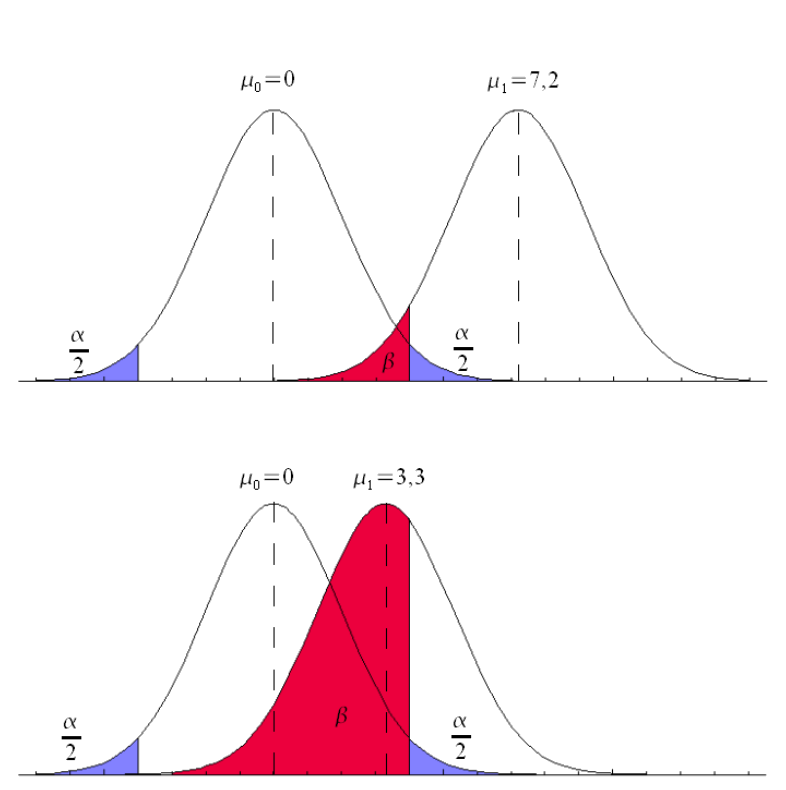
\includegraphics[width=0.6\textwidth]{includes/figures/example_fehler.png}
    \end{center}
\end{example}

\begin{defi}{Operationscharakteristik und Gütefunktion}
    Die \emph{Operationscharakteristik} ist ein Konzept, mit dem ein funktionaler Zusammenhang zwischen der Wahrscheinlichkeit eines Fehlers 2. Art und der tatsächlichen Lage des unbekannten Parameters $\theta$ einer Verteilungsfunktion $F(x \mid \theta)$ hergestellt wird.

    Sei $\theta_1$ der \emph{tatsächliche} Parameter.
    Dann berechnet sich der Fehler 2. Art als Wahrscheinlichkeit, dass ein eine Testvariable $\hat{t}$ in den nicht-kritischen Bereich der Nullhypothese fällt, obwohl in Wahrheit $\theta_1$ statt $\theta_0$ die Verteilung bestimmt:
    \[
        \beta = P (\hat{t} \in \text{nicht-kritischer Bereich von $H_0$} \mid \theta_1)
    \]

    $\beta$ hängt also von $\theta_1$ ab und kann daher als Funktion von $\theta_1$ definiert werden:
    \[
        \beta = f(\theta_1) \quad \text{bzw.} \quad \beta = \beta(\theta_1)
    \]
    Diese Funktion wird als \emph{Operationscharakteristik}, bezeichnet.

    Die Gegenwahrscheinlichkeit zu $\beta$ ist, dass $H_0$ abgelehnt und dafür $H_1$ akzeptiert wird, wenn $\theta_1$ der wahre Parameter ist.

    Hier ist die Ablehnung von $H_0$ zu Gunsten von $H_1$ also erwünscht, weshalb die entsprechende Funktion
    \[
        \gamma(\theta_1) = 1 - \beta(\theta_1)
    \]
    auch \emph{Gütefunktion} genannt wird.
\end{defi}

\begin{algo}{Bestimmung der Grenze bei einem einfachen Alternativtest}
    \begin{itemize}
        \item Nullhypothese $\mhl{H_0: p = p_0}$, Alternativhypothese $\mhl{H_1: p = p_1}$\footnote{Wir nehmen an, $p_1 > p_0$}
        \item Stichprobe des Umfangs $n$
        \item Ergebnis: $N$ Elemente mit relevanter Eigenschaft (z.B. defekte Schrauben in der Stichprobe)
    \end{itemize}

    Gesucht ist eine Signifikantsschranke bzw. Grenze $k$, mit der wir uns bei einem Ergebnis $N$ für $H_0$, bzw. $H_1$ bei einer Stichprobe von $n$ Elementen entscheiden können:
    \[
        N > k \implies \text{Entscheidung für $H_1$} \quad \text{bzw.} \quad N \leq k \implies \text{Entscheidung für $H_0$}
    \]

    Für die Wahrscheinlichkeit für einen Fehler 1. Art gilt (z.B. bei einer Binomialverteilung):
    \[
        \alpha = \alpha(k) = P(N > k \mid p = p_0) = \sum_{l=k+1}^n \binom{n}{l} p_0^l (1-p_0)^{n-l}
    \]

    Für die Wahrscheinlichkeit für einen Fehler 2. Art gilt (z.B. bei einer Binomialverteilung):
    \[
        \beta = \beta(k) = P(N \leq k \mid p = p_1) = \sum_{l=0}^k \binom{n}{l} p_1^l (1-p_1)^{n-l}
    \]
\end{algo}

\begin{algo}{Bestimmung der Grenze bei einem einseitigen Hypothesentest}
    \begin{itemize}
        \item Nullhypothese $\mhl{H_0: p \leq p_0}$, Alternativhypothese $\mhl{H_1: p > p_0}$
        \item Stichprobe des Umfangs $n$
        \item Ergebnis: $N$ Elemente mit relevanter Eigenschaft (z.B. defekte Schrauben in der Stichprobe)
    \end{itemize}

    Gesucht ist eine Signifikantsschranke bzw. Grenze $k$, mit der wir uns bei einem Ergebnis $N$ für $H_0$, bzw. $H_1$ bei einer Stichprobe von $n$ Elementen entscheiden können:
    \[
        N > k \implies \text{Entscheidung für $H_1$} \quad \text{bzw.} \quad N \leq k \implies \text{Entscheidung für $H_0$}
    \]

    Um möglichst selten eine falsche Entscheidung zu treffen, legt man eine obere Schranke $\alpha_0$ für die Fehlerwahrscheinlichkeit 1. Art fest:
    \[
        \alpha \leq \alpha_0
    \]

    Für die Wahrscheinlichkeit für einen Fehler 1. Art gilt (z.B. bei einer Binomialverteilung):
    \[
        \alpha = \alpha(p) = P(N > k \mid p) = \sum_{l=k+1}^n \binom{n}{l} p^l (1-p)^{n-l} \leq \alpha_0 \quad \forall p \leq p_0
    \]

    $\alpha(p)$ ist streng monoton wachsend in $p$.
    Damit gilt:
    \[
        \alpha(p) \leq \alpha(p_0) \quad \forall p \leq p_0
    \]

    Das gesuchte $k$ ist dann das kleinste $k$, das die folgende Ungleichung erfüllt:
    \[
        \sum_{l=k+1}^n \binom{n}{l} p_0^l (1-p_0)^{n-l} \leq \alpha_0
    \]

\end{algo}

\begin{algo}{Bestimmung der Grenzen bei einem zweiseitigen Hypothesentest}
    \begin{itemize}
        \item Nullhypothese $\mhl{H_0: p = p_0}$, Alternativhypothese $\mhl{H_1: p \neq p_0}$
        \item Stichprobe des Umfangs $n$
        \item Ergebnis: $N$ Elemente mit relevanter Eigenschaft (z.B. defekte Schrauben in der Stichprobe)
    \end{itemize}

    Gesucht sind eine Signifikantsschranken bzw. Grenzen $k_1$ und $k_2$, mit denen wir uns bei einem Ergebnis $N$ für $H_0$, bzw. $H_1$ bei einer Stichprobe von $n$ Elementen entscheiden können:
    \[
        N < k_1 \, \lor \, N > k_2 \implies \text{Entscheidung für $H_1$} \quad \text{bzw.} \quad k_1 \leq N \leq k_2 \implies \text{Entscheidung für $H_0$}
    \]

    Um möglichst selten eine falsche Entscheidung zu treffen, legt man eine obere Schranke $\alpha_0$ für die Fehlerwahrscheinlichkeit 1. Art fest:
    \[
        \alpha \leq \alpha_0
    \]

    Für die Wahrscheinlichkeit für einen Fehler 1. Art gilt (z.B. bei einer Binomialverteilung):
    \begin{alignat*}{1}
        \alpha = \alpha(p) & = P(N < k_1 \, \lor \, N > k_2 \mid p = p_0)                                                                                  \\
                           & = \sum_{l=0}^{k_1 - 1} \binom{n}{l} p_0^l (1-p_0)^{n-l} + \sum_{l=k_2 + 1}^{n} \binom{n}{l} p_0^l (1-p_0)^{n-l} \leq \alpha_0
    \end{alignat*}

    Wir müssen die Wahrscheinlichkeiten auf beide Seiten symmetrisch verteilen und erhalten:
    \[
        \sum_{l=0}^{k_1 - 1} \binom{n}{l} p_0^l (1-p_0)^{n-l} \leq \frac{\alpha}{2} \quad \text{mit größten $k_1$}
    \]
    \[
        \sum_{l=k_2 + 1}^{n} \binom{n}{l} p_0^l (1-p_0)^{n-l} \leq \frac{\alpha}{2} \quad \text{mit kleinsten $k_2$}
    \]
\end{algo}

\begin{algo}{Zweiseitiger Einstichproben-Gauß-Test}
    \begin{itemize}
        \item Normalverteilung mit unbekanntem Erwartungswert $\mu$ und bekannter Varianz $\sigma^2$
        \item Nullhypothese $\mhl{H_0: \mu = \mu_0}$, Alternativhypothese $\mhl{H_1: \mu \neq \mu_0}$
        \item Test:
              \[
                  \abs{\conj{X} - \mu_0}
                  \begin{cases}
                      > c    & \implies \text{Entscheidung für $H_1$} \\
                      \leq c & \implies \text{Entscheidung für $H_0$}
                  \end{cases}
              \]
    \end{itemize}

    \begin{enumerate}
        \item Vorgabe des Signifikanzniveaus $\alpha$ (Wahrscheinlichkeit für Fehler 1. Art)
        \item Berechnung der kritischen Grenze $c$ unter der Annahme, dass $H_0$ gültig ist:
              \begin{alignat*}{1}
                  \alpha & = P(\conj{X} - \mu_0 > c) + P(\conj{X} - \mu_0 < -c)                                                                                                                                                     \\
                         & = P \left( \sqrt{n} \cdot \frac{\conj{X} - \mu_0}{\sigma} > \sqrt{n} \cdot \frac{c}{\sigma} \right) + P \left( \sqrt{n} \cdot \frac{\conj{X} - \mu_0}{\sigma} < -\sqrt{n} \cdot \frac{c}{\sigma} \right)
              \end{alignat*}

              Die Variable
              \[
                  u = \sqrt{n} \cdot \frac{\conj{X} - \mu_0}{\sigma}
              \]
              ist standardnormalverteilt.
              Es gilt weiterhin:
              \[
                  \alpha  = 1 - \Phi \left( \sqrt{n} \cdot \frac{c}{\sigma} \right) + \Phi \left( \sqrt{n} \cdot \frac{-c}{\sigma} \right) = 2 - 2 \cdot \Phi \left( \sqrt{n} \cdot \frac{c}{\sigma} \right)
              \]
              \[
                  \implies  \Phi \left( \sqrt{n} \cdot \frac{c}{\sigma} \right) = 1 - \frac{\alpha}{2} \implies  \sqrt{n} \cdot \frac{c}{\sigma} = u_{1 - \nicefrac{\alpha}{2}} \implies  c = u_{1 - \nicefrac{\alpha}{2}} \cdot \frac{\sigma}{\sqrt{n}}
              \]
        \item Testentscheidung:
              \[
                  \abs{\conj{X} - \mu_0}
                  \begin{cases}
                      \mhl{ > u_{1 - \nicefrac{\alpha}{2}} \cdot \frac{\sigma}{\sqrt{n}} }     & \implies \text{Entscheidung für $H_1$} \\
                      \mhl{ \leq u_{1 - \nicefrac{\alpha}{2}}  \cdot \frac{\sigma}{\sqrt{n}} } & \implies \text{Entscheidung für $H_0$}
                  \end{cases}
              \]
        \item Gütefunktion:
              \begin{alignat*}{1}
                  \gamma(\mu) & = P(\conj{X} - \mu_0 > c) + P(\conj{X} - \mu_0 < -c) = P(\conj{X} > c + \mu_0) + P(\conj{X} < -c + \mu_0)                                                                                                                      \\
                              & = P \left( \sqrt{n} \cdot \frac{\abs{X} - \mu}{\sigma} > \sqrt{n} \cdot \frac{c + \mu_0 - \mu}{\sigma} \right) + P \left( \sqrt{n} \cdot \frac{\abs{X} - \mu}{\sigma} < \sqrt{n} \cdot \frac{-c + \mu_0 - \mu}{\sigma} \right) \\
                              & = 1 - \Phi \left( \sqrt{n} \cdot \frac{c + \mu_0 - \mu}{\sigma} \right) + \Phi \left( \sqrt{n} \cdot \frac{-c + \mu_0 - \mu}{\sigma} \right)                                                                                   \\
                              & = 1 - \Phi \left( \sqrt{n} \cdot \frac{c}{\sigma} + \frac{\sqrt{n}}{\sigma} \cdot (\mu_0 - \mu) \right) + \Phi \left( \sqrt{n} \cdot \frac{-c}{\sigma} + \frac{\sqrt{n}}{\sigma} \cdot (\mu_0 - \mu) \right)                   \\
                              & = \mhl{ 1 - \Phi \left( u_{1 - \nicefrac{\alpha}{2}} + \frac{\sqrt{n}}{\sigma} \cdot (\mu_0 - \mu) \right) + \Phi \left( -u_{1 - \nicefrac{\alpha}{2}} + \frac{\sqrt{n}}{\sigma} \cdot (\mu_0 - \mu) \right) }
              \end{alignat*}
    \end{enumerate}
\end{algo}

\begin{defi}{Konsistenz eines Tests}
    Bei ausreichend großen Stichprobenumfängen wird $H_0$ immer abgelehnt, falls dies berechtigt ist.
    Mit wachsendem Stichprobenumfang wächst also die Wahrscheinlichkeit, einen Fehler 2. Art zu vermeiden.
    Der Parametertest heißt \emph{konsistent}.
\end{defi}

\begin{algo}{Berechnung des Mindeststichprobenumfangs}
    \begin{itemize}
        \item Signifikanzniveau $\alpha$
        \item Wert $\mu = \mu_1$
    \end{itemize}

    Gesucht sei der Mindeststichprobenumfang $n_0$ so, dass damit die Wahrscheinlichkeit für den Fehler 2. Art höchstens
    \[
        \beta_0 = \beta(\mu_1)
    \]
    ist. Typisch sind z.B. $\alpha = 0.01$ und $\beta_0 = 0.1$.

    Es gilt für einen \emph{zweiseitigen Test}:
    \[
        n_0 = (u_{1 - \nicefrac{\alpha}{2}} + u_{1 - \beta_0}) ^2 \cdot \frac{\sigma^2}{(\mu_1 - \mu_0)^2}
    \]

    Bei den typischen Werten $\alpha = 0.01$ und $\beta_0 = 0.1$ gilt vereinfacht:
    \[
        n = 14.88 \cdot \frac{\sigma^2}{(\mu_1 - \mu_0)^2} \approx \mhl{15 \cdot \frac{\sigma^2}{(\mu_1 - \mu_0)^2}}
    \]

    Es gilt für einen \emph{einseitigen Test}:
    \[
        n_0 = (u_{1 - \alpha} + u_{1 - \beta_0}) ^2 \cdot \frac{\sigma^2}{(\mu_1 - \mu_0)^2}
    \]

    Bei den typischen Werten $\alpha = 0.01$ und $\beta_0 = 0.1$ gilt vereinfacht:
    \[
        n = 13.02 \cdot \frac{\sigma^2}{(\mu_1 - \mu_0)^2} \approx \mhl{15 \cdot \frac{\sigma^2}{(\mu_1 - \mu_0)^2}}
    \]

\end{algo}

\begin{algo}{Einseitiger Einstichproben-Gauß-Test (Abgrenzung nach oben)}
    \begin{itemize}
        \item Normalverteilung mit unbekanntem Erwartungswert $\mu$ und bekannter Varianz $\sigma^2$
        \item Nullhypothese $\mhl{H_0: \mu \leq \mu_0}$, Alternativhypothese $\mhl{H_1: \mu > \mu_0}$
    \end{itemize}
    \[
        \abs{\conj{X} - \mu_0}
        \begin{cases}
            > c    & \implies \text{Entscheidung für $H_1$} \\
            \leq c & \implies \text{Entscheidung für $H_0$}
        \end{cases}
    \]

    \begin{enumerate}
        \item Vorgabe des Signifikanzniveaus $\alpha$ (Wahrscheinlichkeit für Fehler 1. Art)
        \item Berechnung der kritischen Grenze $c$ unter der Annahme, dass $H_0$ gültig ist:
              \[
                  1 - \alpha = P(\conj{X} - \mu_0 \leq c) = P \left( \sqrt{n} \cdot \frac{\conj{X} - \mu_0}{\sigma} \leq \sqrt{n} \cdot \frac{c}{\sigma} \right)
              \]

              Die Variable
              \[
                  u = \sqrt{n} \cdot \frac{\conj{X} - \mu_0}{\sigma}
              \]
              ist standardnormalverteilt.
              Es gilt weiterhin:
              \[
                  1 - \alpha = \Phi \left( \sqrt{n} \cdot \frac{c}{\sigma} \right) \quad \implies \quad \sqrt{n} \cdot \frac{c}{\sigma} = u_{1 - \alpha} \quad \implies \quad c = u_{1 - \alpha} \cdot \frac{\sigma}{\sqrt{n}}
              \]
        \item Testentscheidung:
              \[
                  \abs{\conj{X} - \mu_0}
                  \begin{cases}
                      \mhl{ > u_{1 - \alpha} \cdot \frac{\sigma}{\sqrt{n}}}    & \implies \text{Entscheidung für $H_1$} \\
                      \mhl{ \leq u_{1 - \alpha} \cdot \frac{\sigma}{\sqrt{n}}} & \implies \text{Entscheidung für $H_0$}
                  \end{cases}
              \]
    \end{enumerate}
\end{algo}

\begin{algo}{Einseitiger Einstichproben-Gauß-Test (Abgrenzung nach unten)}
    \begin{itemize}
        \item Normalverteilung mit unbekanntem Erwartungswert $\mu$ und bekannter Varianz $\sigma^2$
        \item Nullhypothese $H_0$: $\mu \geq \mu_0$, Alternativhypothese $H_1$: $\mu < \mu_0$
    \end{itemize}
    \[
        \abs{\conj{X} - \mu_0}
        \begin{cases}
            < c    & \implies \text{Entscheidung für $H_1$} \\
            \geq c & \implies \text{Entscheidung für $H_0$}
        \end{cases}
    \]

    \begin{enumerate}
        \item Vorgabe des Signifikanzniveaus $\alpha$ (Wahrscheinlichkeit für Fehler 1. Art)
        \item Berechnung der kritischen Grenze $c$ unter der Annahme, dass $H_0$ gültig ist:
              \[
                  \alpha = P(\conj{X} - \mu_0 \leq c) = P \left( \sqrt{n} \cdot \frac{\conj{X} - \mu_0}{\sigma} \leq \sqrt{n} \cdot \frac{c}{\sigma} \right)
              \]

              Die Variable
              \[
                  u = \sqrt{n} \cdot \frac{\conj{X} - \mu_0}{\sigma}
              \]
              ist standardnormalverteilt.
              Es gilt weiterhin:
              \[
                  \alpha = \Phi \left( \sqrt{n} \cdot \frac{c}{\sigma} \right) \quad \implies \quad \sqrt{n} \cdot \frac{c}{\sigma} = u_{\alpha} \quad \implies \quad c = u_{\alpha} \cdot \frac{\sigma}{\sqrt{n}}
              \]
        \item Testentscheidung:\footnote{Es gilt $\abs{u_{1 - \alpha}} = \abs{u_{\alpha}}$}
              \[
                  \abs{\conj{X} - \mu_0}
                  \begin{cases}
                      \mhl{ < u_{1 - \alpha} \cdot \frac{\sigma}{\sqrt{n}}   } & \implies \text{Entscheidung für $H_1$} \\
                      \mhl{ \geq u_{1 - \alpha} \cdot \frac{\sigma}{\sqrt{n}}} & \implies \text{Entscheidung für $H_0$}
                  \end{cases}
              \]
    \end{enumerate}
\end{algo}

\begin{bonus}{Zusammenfassung Einstichproben-Gauß-Test}
    \begin{center}
        \begin{tabular}{|c|c|c|}
            \hline
            $H_0$                          & $H_1$                             & Kritischer Bereich für Signifikanzniveau $\alpha$                                                                    \\
            \hline
            \multirow{2}{*}{$\mu = \mu_0$} & \multirow{2}{*}{$\mu \neq \mu_0$} & \multirow{2}{*}{$\displaystyle \sqrt{n} \cdot \frac{\abs{\conj{X} - \mu_0}}{\sigma} > u_{1 - \nicefrac{\alpha}{2}}$} \\
                                           &                                   &                                                                                                                      \\
            \hline
            $\mu \geq \mu_0$               & $\mu < \mu_0$                     & \multirow{2}{*}{$\displaystyle \sqrt{n} \cdot \frac{\abs{\conj{X} - \mu_0}}{\sigma} > u_{1 - \alpha}$}               \\
            $\mu \leq \mu_0$               & $\mu > \mu_0$                     &                                                                                                                      \\
            \hline
        \end{tabular}
    \end{center}
\end{bonus}

\begin{algo}{Zweiseitiger Einstichproben-t-Test}
    \begin{itemize}
        \item Normalverteilung mit unbekanntem Erwartungswert $\mu$ und unbekannter Varianz $\sigma^2$
        \item Nullhypothese $\mhl{H_0: \mu = \mu_0}$, Alternativhypothese $\mhl{H_1: \mu \neq \mu_0}$
    \end{itemize}

    \begin{enumerate}
        \item Vorgabe des Signifikanzniveaus $\alpha$ (Wahrscheinlichkeit für Fehler 1. Art)
        \item Berechnung der Test- oder Prüfvariablen:
              \[
                  T = \sqrt{n} \cdot \frac{\conj{X} - \mu_0}{S}
              \]
              ist t-verteilt mit $f = n-1$ Freiheitsgraden.

              Es gilt weiterhin:
              \[
                  1 - \alpha = P(-c \leq T \leq c) \quad \implies \quad c = t_{n-1} (1 - \nicefrac{\alpha}{2})
              \]
        \item Testentscheidung anhand eines konkreten Stichprobenergebnisses
              \[
                  \hat{t} = \sqrt{n} \cdot \frac{\conj{X} - \mu_0}{S}
              \]
              \[
                  \abs{\hat{t}}
                  \begin{cases}
                      \mhl{ > t_{n-1} (1 - \nicefrac{\alpha}{2}) }    & \implies \text{Entscheidung für $H_1$} \\
                      \mhl{ \leq t_{n-1} (1 - \nicefrac{\alpha}{2}) } & \implies \text{Entscheidung für $H_0$}
                  \end{cases}
              \]
    \end{enumerate}
\end{algo}

\begin{algo}{Einseitiger Einstichproben-t-Test (Abgrenzung nach oben)}
    \begin{itemize}
        \item Normalverteilung mit unbekanntem Erwartungswert $\mu$ und unbekannter Varianz $\sigma^2$
        \item Nullhypothese $\mhl{H_0: \mu \leq \mu_0}$, Alternativhypothese $\mhl{H_1: \mu > \mu_0}$
    \end{itemize}
    \[
        \abs{\conj{X} - \mu_0}
        \begin{cases}
            > c    & \implies \text{Entscheidung für $H_1$} \\
            \leq c & \implies \text{Entscheidung für $H_0$}
        \end{cases}
    \]

    \begin{enumerate}
        \item Vorgabe des Signifikanzniveaus $\alpha$ (Wahrscheinlichkeit für Fehler 1. Art)
        \item Berechnung der Test- oder Prüfvariablen:
              \[
                  T = \sqrt{n} \cdot \frac{\conj{X} - \mu_0}{S}
              \]
              ist t-verteilt mit $f = n-1$ Freiheitsgraden.

              Es gilt weiterhin:
              \[
                  1 - \alpha = P(T \leq c) \quad \implies \quad c = t_{n-1} (1 - \alpha)
              \]
        \item Testentscheidung anhand eines konkreten Stichprobenergebnisses
              \[
                  \hat{t} = \sqrt{n} \cdot \frac{\conj{X} - \mu_0}{S}
              \]
              \[
                  \abs{\hat{t}}
                  \begin{cases}
                      \mhl{ > t_{n-1} (1 - \alpha) }   & \implies \text{Entscheidung für $H_1$} \\
                      \mhl{ \leq t_{n-1} (1 - \alpha)} & \implies \text{Entscheidung für $H_0$}
                  \end{cases}
              \]
    \end{enumerate}
\end{algo}

\begin{algo}{Einseitiger Einstichproben-t-Test (Abgrenzung nach unten)}
    \begin{itemize}
        \item Normalverteilung mit unbekanntem Erwartungswert $\mu$ und unbekannter Varianz $\sigma^2$
        \item Nullhypothese $\mhl{H_0: \mu \geq \mu_0}$, Alternativhypothese $\mhl{H_1: \mu < \mu_0}$
    \end{itemize}
    \[
        \abs{\conj{X} - \mu_0}
        \begin{cases}
            < c    & \implies \text{Entscheidung für $H_1$} \\
            \geq c & \implies \text{Entscheidung für $H_0$}
        \end{cases}
    \]

    \begin{enumerate}
        \item Vorgabe des Signifikanzniveaus $\alpha$ (Wahrscheinlichkeit für Fehler 1. Art)
        \item Berechnung der Test- oder Prüfvariablen:
              \[
                  T = \sqrt{n} \cdot \frac{\conj{X} - \mu_0}{S}
              \]
              ist t-verteilt mit $f = n-1$ Freiheitsgraden.

              Es gilt weiterhin:
              \[
                  1 - \alpha = P(T \geq c) \quad \implies \quad c = t_{n-1} (\alpha)
              \]
        \item Testentscheidung anhand eines konkreten Stichprobenergebnisses\footnote{Es gilt: $\abs{t_{n-1} (\alpha)} = \abs{t_{n-1} (1-\alpha)}$}
              \[
                  \hat{t} = \sqrt{n} \cdot \frac{\conj{X} - \mu_0}{S}
              \]
              \[
                  \abs{\hat{t}}
                  \begin{cases}
                      \mhl{ < t_{n-1} (\alpha)  }  & \implies \text{Entscheidung für $H_1$} \\
                      \mhl{ \geq t_{n-1} (\alpha)} & \implies \text{Entscheidung für $H_0$}
                  \end{cases}
              \]
    \end{enumerate}
\end{algo}

\begin{bonus}{Zusammenfassung Einstichproben-t-Test}
    \begin{center}
        \begin{tabular}{|c|c|c|}
            \hline
            $H_0$                          & $H_1$                             & Kritischer Bereich für Signifikanzniveau $\alpha$                                                                     \\
            \hline
            \multirow{2}{*}{$\mu = \mu_0$} & \multirow{2}{*}{$\mu \neq \mu_0$} & \multirow{2}{*}{$\displaystyle \sqrt{n} \cdot \frac{\abs{\conj{X} - \mu_0}}{S} > t_{n-1} (1 - \nicefrac{\alpha}{2})$} \\
                                           &                                   &                                                                                                                       \\
            \hline
            $\mu \geq \mu_0$               & $\mu < \mu_0$                     & \multirow{2}{*}{$\displaystyle \sqrt{n} \cdot \frac{\abs{\conj{X} - \mu_0}}{S} > t_{n-1} (1 - \alpha)$}               \\
            $\mu \leq \mu_0$               & $\mu > \mu_0$                     &                                                                                                                       \\
            \hline
        \end{tabular}
    \end{center}
\end{bonus}

